% ===========================================================================
\section{Farey 序列}\label{sec:farey}

Farey 序列与 Stern--Brocot 树共享同一套中位分数结构，只是把``树''压平成
``分母有界的分数列表''。

\subsection{定义与基本性质}

\begin{definition}[Farey 序列]
第 $n$ 阶 \keyword{Farey 序列} $F_n$ 是 $[0,1]$ 中所有分母不超过 $n$ 的最简分数
按大小排列的序列：
\[
  F_1=\Big(\frac01,\frac11\Big),\quad
  F_2=\Big(\frac01,\frac12,\frac11\Big),\quad
  F_3=\Big(\frac01,\frac13,\frac12,\frac23,\frac11\Big),\quad
  F_4=\Big(\frac01,\frac14,\frac13,\frac12,\frac23,\frac34,\frac11\Big).
\]
\end{definition}

\begin{proposition}\label{prop:farey-sub}
$F_n$ 是在 $F_{n-1}$ 的某些相邻分数之间插入中位分数得到的：$F_n\setminus F_{n-1}$
恰为分母等于 $n$ 的最简分数。等价地，$F_n$ 是第 $n-1$ 阶 Stern--Brocot 序列
（限制在 $[0,1]$ 内）按``分母 $\le n$''筛出的子序列。
\end{proposition}

\begin{proof}
分母 $\le n$ 的最简分数都在 Stern--Brocot 树上（定理 \ref{thm:complete}），且树
的中序遍历单调（命题 \ref{prop:monotone}），故按大小排列就是按中序顺序取出；
分母恰为 $n$ 的分数不在 $F_{n-1}$ 中，其分子与 $n$ 互素。插入位置的正确性由
分母引理（引理 \ref{lem:denominator}）保证：分母为 $b+d$ 的中位分数是其端点间
分母最小的分数，所以在 $F_{b+d-1}$ 及以前端点仍相邻。
\end{proof}

\begin{corollary}[长度公式]\label{cor:farey-length}
记 $\varphi$ 为 Euler 函数，则
\[
  |F_n|=|F_{n-1}|+\varphi(n)=1+\sum_{k=1}^{n}\varphi(k).
\]
\end{corollary}

\begin{proof}
$F_n$ 相对 $F_{n-1}$ 新增的分数分母都是 $n$，分子取遍 $\{1,\ldots,n\}$ 中与 $n$
互素的数，恰 $\varphi(n)$ 个；初值 $|F_1|=2$，而求和约定从 $\varphi(1)=1$ 起
计入端点 $1/1$，写成上式。
\end{proof}

\subsection{Farey 邻项}

\begin{definition}[Farey 邻项]
若分数 $a/b$ 与 $c/d$ 在某个 Farey 序列中相邻，则称它们为一对
\keyword{Farey 邻项}（Farey neighbors）。
\end{definition}

\begin{theorem}[Farey 邻项的刻画]\label{thm:farey-neighbor}
设 $a/b<c/d$ 为 $[0,1]$ 中的最简分数。则以下两条等价：
\begin{enumerate}[label=(\roman*)]
  \item $a/b$ 与 $c/d$ 是 Farey 邻项；
  \item $bc-ad=1$。
\end{enumerate}
此外，它们在 $F_{\max(b,d)},F_{\max(b,d)+1},\ldots,F_{b+d-1}$ 中都相邻，并在
$F_{b+d}$ 中被它们的中位分数分开。特别地，$a/b$ 与 $c/d$ 在 $F_N$ 中相邻，
当且仅当 $bc-ad=1$ 且 $b+d>N$。
\end{theorem}

\begin{proof}
(i)$\Rightarrow$(ii)：Farey 邻项在某个 $F_n$ 中相邻。由命题
\ref{prop:farey-sub}，两分数中后加入者是另一者与它先前邻项的中位分数，故两者
在某阶 Stern--Brocot 序列中也相邻；由行列式不变量（命题 \ref{prop:invariant}），
Stern--Brocot 序列中相邻分数满足 $bc-ad=1$。

(ii)$\Rightarrow$(i)：不妨设 $b\ge d$（$b$ 为较大的分母），则两分数都属于
$F_b$。设 $e/f$ 是 $F_b$ 中紧接在 $a/b$ 右侧的分数，由已证的必要性知
$be-af=1$。考虑线性 Diophantine 方程
\[
  bx-ay=1.
\]
其通解由任一特解加上 $(a,b)$ 的整数倍得到，故满足 $0<y\le b$ 的解\emph{唯一}。
条件 $bc-ad=1$ 表明 $(x,y)=(c,d)$ 就是这样一组解（$d\le b$），而 $(e,f)$ 也是，
故 $(e,f)=(c,d)$，即 $c/d$ 就是 $a/b$ 在 $F_b$ 中的右邻。

最后，第一个严格落在两者之间且分母最小的分数是中位分数 $(a+c)/(b+d)$
（引理 \ref{lem:denominator}），它出现在 $F_{b+d}$ 中；此前两者一直保持相邻。
$b+d>N$ 的刻画随之而得。
\end{proof}

\begin{corollary}[邻项总数]
$F_n$ 中 Farey 邻项共 $2|F_n|-3$ 对（按``在某个 $F_n$ 中相邻且分母均不超过
$n$''计数）。
\end{corollary}

\begin{proof}
除端点 $0/1$ 与 $1/1$ 外，每个 $p/q\in F_n$（$q\ge2$）的左、右邻项由方程
$qx-py=\pm1$ 在 $y<q$ 范围内的唯一解给出，各对应一个分母更小的邻项；每个分数
贡献两对，而 $0/1$ 与 $1/1$ 之间只有一对。合计 $2(|F_n|-2)+1=2|F_n|-3$。
\end{proof}

\begin{remark}[求指定分数的邻项]
对给定的 $p/q=[t_0;t_1,\ldots,t_n,1]$，插入它时它左右两侧的邻项（即分母更小
的两个 Farey 邻项）分别是 $[t_0;t_1,\ldots,t_n]$ 与 $[t_0;t_1,\ldots,t_n-1]$。
全部分母不超过某界的邻项可由扩展 Euclid 算法解 $qx-py=\pm1$ 得到。
\end{remark}

\subsection{Ford 圆}

Farey 邻项有一个漂亮的几何等价刻画。

\begin{definition}[Ford 圆]
对每个 $[0,1]$ 内的最简分数 $p/q$，以 $\Big(\dfrac pq,\dfrac{1}{2q^2}\Big)$ 为
圆心、$\dfrac{1}{2q^2}$ 为半径作圆，称为 $p/q$ 的 \keyword{Ford 圆}。这些圆都
与 $x$ 轴相切于 $(p/q,0)$，如图 \ref{fig:ford} 所示。
\end{definition}

\begin{figure}[htbp]
\centering
\begin{tikzpicture}
  \node[inner sep=0pt] (img)
    {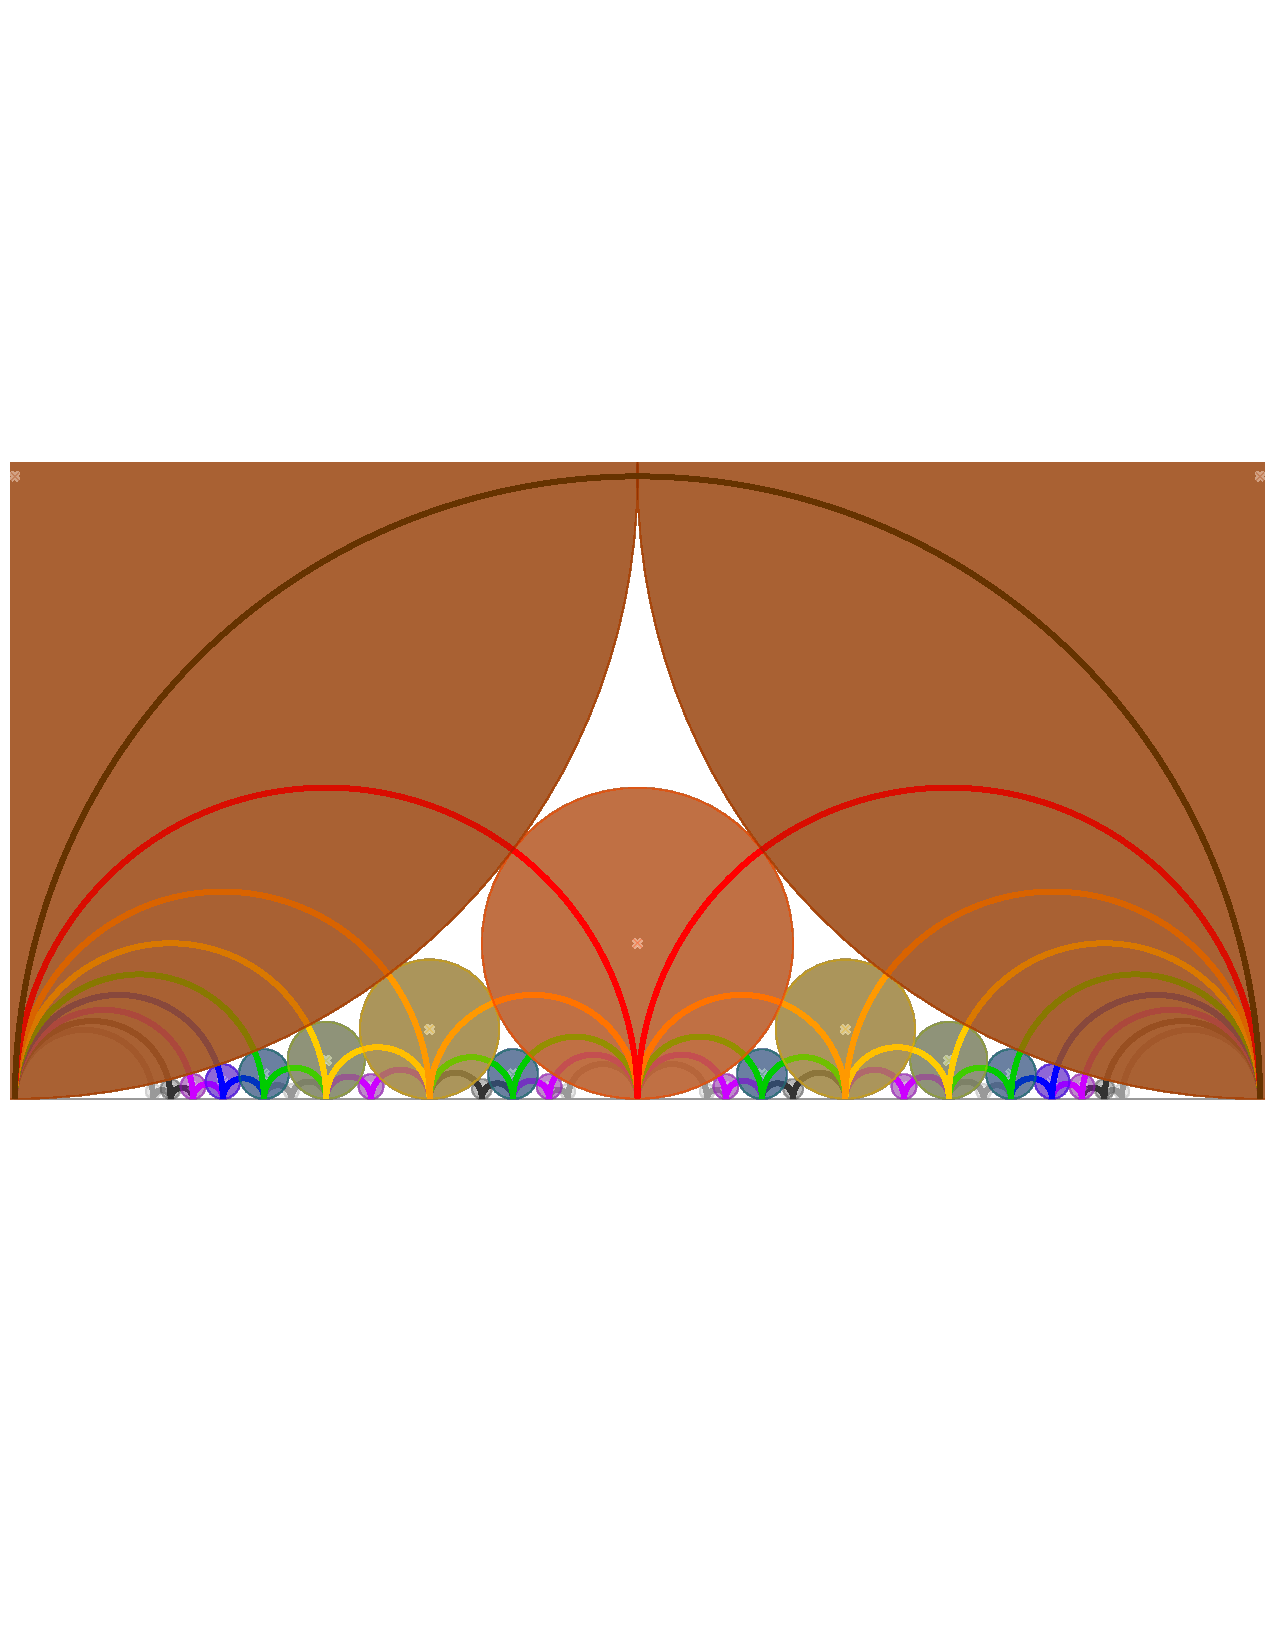
\includegraphics[width=\textwidth]{ford-circles.pdf}};
  % 分数 p/q 的切点位于图宽约 0.0033+0.9934*(p/q) 处
  \foreach \p/\q in {0/1, 1/6, 1/5, 1/4, 1/3, 2/5, 1/2, 3/5, 2/3, 3/4, 4/5, 5/6, 1/1}{
    \pgfmathsetmacro{\fx}{0.0033+0.9934*(\p/\q)}
    \coordinate (t) at ($(img.south west)!\fx!(img.south east)$);
    \draw[selvage, thin] (t) -- ++(0,-1.5pt);
    \node[below=3pt, font=\footnotesize] at (t) {$\frac{\p}{\q}$};
  }
\end{tikzpicture}
\caption{$F_1$ 至 $F_9$ 各分数的 Ford 圆与 Farey 弧线对照图。每个 Ford 圆与
$x$ 轴相切于对应分数处；两圆外切当且仅当对应分数是 Farey 邻项（定理
\ref{thm:ford}）。图中同色的半圆弧是 Farey 图中连接相邻分数的弧线，每条弧与
对应的 Ford 圆正交。原图底部的交互式标注在静态打印时会互相重叠，本笔记将其
隐去，改标 $F_6$ 的十三个分数（更密的标注在本图宽度下无法避免重叠，这正是
原图采用悬停交互的原因）。原图：CMG Lee，Wikimedia Commons，CC BY-SA 4.0
（有改动：去除标注层、转为 PDF 并裁剪）。}
\label{fig:ford}
\end{figure}

\begin{theorem}[Ford 圆与 Farey 邻项]\label{thm:ford}
两个不同的最简分数 $a/b<c/d$ 的 Ford 圆只可能相切或相离；它们相切，当且仅当
$|bc-ad|=1$，即两分数是 Farey 邻项。此时存在唯一的第三个 Ford 圆与两圆都相切，
它对应的分数恰是中位分数 $(a+c)/(b+d)$。
\end{theorem}

\begin{proof}
计算两圆心距离的平方与半径和、差的平方：
\[
  \Big(\frac ab-\frac cd\Big)^2+\Big(\frac{1}{2b^2}-\frac{1}{2d^2}\Big)^2
  =\Big(\frac{1}{2b^2}+\frac{1}{2d^2}\Big)^2+\frac{(bc-ad)^2-1}{b^2d^2}.
\]
两分数不同且都最简，故 $bc-ad$ 是非零整数，$|bc-ad|\ge1$，于是圆心距不小于半径
之和，即两圆相离或外切；取等号（外切）当且仅当 $|bc-ad|=1$，由定理
\ref{thm:farey-neighbor} 这等价于 Farey 邻项。相切时中位分数的圆与两者都相切
（因中位分数与每个端点都满足行列式 $1$ 的关系），唯一性由两圆公切圆在
$x$ 轴切点位置的唯一性给出。
\end{proof}

\subsection{递推关系}

Farey 序列可以自左向右递推生成，无需逐一插入。

\begin{proposition}[Farey 序列的三项递推]\label{prop:farey-recurrence}
设 $F_n$ 中相邻三项为 $\dfrac ab<\dfrac pq<\dfrac cd$，则存在整数 $k\ge1$ 使
\[
  a+c=kp,\qquad b+d=kq,
\]
且 $k$ 由
\[
  k=\Big\lfloor\frac{n+b}{q}\Big\rfloor
\]
唯一确定。由此，记 $F_n$ 的第 $i$ 项为 $p_i/q_i$，则
\[
  p_{i}=\Big\lfloor\frac{n+q_{i-2}}{q_{i-1}}\Big\rfloor p_{i-1}-p_{i-2},
  \qquad
  q_{i}=\Big\lfloor\frac{n+q_{i-2}}{q_{i-1}}\Big\rfloor q_{i-1}-q_{i-2},
\]
递推起点为 $(p_0,q_0)=(0,1)$，$(p_1,q_1)=(1,n)$。
\end{proposition}

\begin{proof}
由定理 \ref{thm:farey-neighbor}，相邻两对都满足行列式关系：
$bp-aq=1=cq-dp$，解出
\[
  \frac pq=\frac{a+c}{b+d}
\]
（中位分数关系，但 $a+c$ 与 $b+d$ 可能有公因子，故写成整数倍 $k$）。于是
$c=kp-a$，$d=kq-b$。$c/d$ 要落在 $F_n$ 中需 $d=kq-b\le n$，即
$k\le(n+b)/q$；而差值
\[
  \frac{kp-a}{kq-b}-\frac pq=\frac{bp-aq}{q(kq-b)}=\frac{1}{q(kq-b)}
\]
随 $k$ 增大而严格减小。$c/d$ 是 $p/q$ 在 $F_n$ 中的\emph{右邻}，即所有满足
$kq-b\le n$ 的候选中差值最小者，故应取最大的可行 $k$，即
$k=\lfloor(n+b)/q\rfloor$。代入 $c=kp-a$、$d=kq-b$ 得递推式；起点 $0/1$ 与
$1/n$ 是 $F_n$ 的前两项。
\end{proof}
